\documentclass[twocolumn]{article}

\usepackage{geometry}
\geometry{textwidth = 18cm,textheight = 24cm}

\usepackage{cite}
\usepackage[utf8]{inputenc}
\usepackage{multirow}
\usepackage{graphicx}
\usepackage{outlines}
\usepackage[dvipsnames]{xcolor}
\usepackage{textcomp}
\usepackage{float}
\usepackage{ulem}
\usepackage{comment}

\usepackage{hyperref}
\hypersetup{
    citecolor = red,
    filecolor = green,
    urlcolor = orange,
    colorlinks = true, %set true if you want colored links
    linktoc = all,     %set to all if you want both sections and subsections linked
    linkcolor = blue,  %choose some color if you want links to stand out
}

%\title{Comparison of semiconductor and superconductor hardware for large-scale optoelectronic neural systems}
\title{Considerations for neuromorphic supercomputing in semiconducting and superconducting optoelectronic hardware}
\author{Bryce A. Primavera and Jeffrey M. Shainline}
\date{April 2021}

\begin{document}

\twocolumn[
\begin{@twocolumnfalse}
\maketitle
\begin{abstract}
Any large-scale neuromorphic system striving for complexity at the level of the human brain and beyond will need to be co-optimized for communication and computation. Such reasoning leads to the proposal for optoelectronic neuromorphic platforms that leverage the complementary properties of optics and electronics. Starting from the conjecture that future large-scale neuromorphic systems will utilize integrated photonics and fiber optics for communication in conjunction with analog electronics for computation, we consider two possible paths towards achieving this vision. The first is a semiconductor platform based on analog CMOS circuits and waveguide-integrated photodiodes. The second is a superconducting approach that utilizes Josephson junctions and waveguide-integrated superconducting single-photon detectors. We discuss available devices, assess scaling potential, and provide a list of key metrics and demonstrations for each platform. Ultimately, both platforms hold potential, but their development will diverge in important respects. Semiconductor systems benefit from a robust fabrication ecosystem and can build on extensive progress made in purely electronic neuromorphic computing, but will require III-V \textcolor{ForestGreen}{light-source} integration \textcolor{ForestGreen}{with electronics} at an unprecedented scale, \sout{continuing development of} \textcolor{ForestGreen}{further advances in} ultra-low capacitance photodiodes, and \sout{exploration of} \textcolor{ForestGreen}{success from} emerging memory technologies. In contrast, superconducting systems place near theoretically minimum burdens on light-sources (a tremendous boon to one of the most speculative aspects of either platform) and provide new opportunities for integrated, high-endurance synaptic memory. However, superconducting optoelectronic systems will also contend with interfacing low-voltage electronic circuits to semiconductor light-sources, the serial biasing of superconducting devices on an unprecedented scale, a less mature fabrication infrastructure, \textcolor{ForestGreen}{and infrastructure challenges associated with cryogenic operation}. 
\vspace{2em}
\end{abstract}
\end{@twocolumnfalse}
]

\setcounter{tocdepth}{4}
\setcounter{secnumdepth}{4}

\section{\label{sec:introduction}Introduction}
The foundations of cognition remain a great frontier of science, with potentially enormous ramifications for technology and society. A platform capable of \sout{simulating} neural function with the scale \textcolor{ForestGreen}{and complexity} of the brain or even beyond could be a powerful tool in \sout{unravelling} \textcolor{ForestGreen}{deciphering} this \sout{great mystery} \textcolor{ForestGreen}{enigma}. Achieving such large-scale systems has proven to be non-trivial with established CMOS hardware \cite{furber2016large}. A significant challenge will be to enable efficient communication with low-latency amongst billions or trillions of neurons. Optics appears well-matched to the task, as the lack of resistive, capacitive, and inductive parasitics makes optical links more amenable to high fan-out than electrical interconnects \cite{shainline2019superconducting}. This eliminates the need for time-multiplexing, allowing direct connections between neurons that will not suffer from the traffic induced delays that \sout{plague} \textcolor{ForestGreen}{limit} neuromorphic systems using digital communication infrastructures \cite{young2019review}, and \sout{paves the way for} \textcolor{ForestGreen}{physically enables} larger, faster, and more interconnected networks. However, while the lack of interaction between photons is beneficial for reducing parasitics during communication, it is a detriment to computation. Electronic circuits are thus better suited to implement complex, nonlinear neuronal functions. \textcolor{ForestGreen}{It is reasonable to anticipate performance gains from optoelectronic neural systems leveraging optics for communication and electronics for computation, provided the hardware can be realized.} \sout{Future neuromorphic systems can therefore be expected to be optoelectronic \textemdash leveraging optics for communication and electronics for computation.}

\begin{figure*}
    \centering
    \includegraphics[scale=1]{_Schematic.pdf}
    \caption{An abstract schematic of the class of optoelectronic neurons meeting our three criteria. Each synapse ($S_e$ and $S_i$ for expiatory and inhibitory synapses respectively) is implemented with a physical circuit block containing a detector and a temporal filter. The detector produces an all-or-nothing electrical pulse upon receipt of an optical spike which is then processed by the filter. The parameters of the filter (time constant, weight, etc.) can be set individually for each synapse. A local weight update circuit (W) implements plasticity mechanisms at each synapse. Synaptic outputs are integrated in the soma (N) which drives an optical transmitter to downstream connections upon reaching threshold.}
    \label{fig:Schematic}
\end{figure*}

Our proposal to fabricate a direct, physical connection between every pair of connected neurons is known as the fully dedicated axon approach to communication \cite{seda2016}. We further specify that all synapses, dendrites, and neurons will utilize fully dedicated electronic circuits as well, so that each element of hardware has a one-to-one correspondence with its information-processing role in the neural system. This stands in contrast to several proposed optoelectronic systems that intend to perform fan-in optically using a shared synapse \cite{nazirzadeh2018energy}. We believe this is necessary to create a diverse array of synaptic behavior at each neuron, as inspired by neuroscience. For instance, a different time constant or plasticity mechanism could be implemented at every synapse on a single neuron. Further, performing weighting in the electronic domain allows for binary optical communication. This minimizes the amount of optical energy per spike and reduces noise incurred by communication. Our thinking can be summarized in the following three points, and the scope of this paper will from hereon be limited to networks meeting these conditions:

\begin{enumerate}
    \item Direct, optical connections are utilized for communication between neurons (fully dedicated axons).
    \item Optical communication is binary. The amplitude of the optical signal carries no information.
    \item All synaptic, dendritic, and somatic computations are performed by fully dedicated electronic circuits.
\end{enumerate}

With these general axioms established, a picture of the hardware under consideration begins to emerge. There is a single optical transmitter at each neuron. This light emitter produces a short pulse of light each time the neuron spikes. The optical pulse is coupled into a waveguide, and optical power is tapped from the waveguide for each downstream synapse. Each synapse contains a photodetector which registers an all-or-nothing synapse event. From there, all synaptic weighting, spike-train filtering, dendritic processing, signal summation, neuronal thresholding, and plasticity mechanisms are implemented in the electronic domain with tailored integrated circuits. A schematic of this general framework is shown in figure \ref{fig:Schematic}.

There are likely many ways to physically implement this model. The remainder of this paper will discuss two possible implementations \textemdash a superconducting platform and a room-temperature all-semiconductor system. The superconducting platform, known as SOENs (Superconducting OptoElectronic Networks) is thoroughly discussed in references \cite{shainline2017superconducting, shainline2019superconducting, shainline2019fluxonic}. In short, optical links are formed from semiconductor light sources and superconducting nanowire single photon detectors (SNSPDs). Computation is performed with analog Josephson junction (JJ) circuits and memory is implemented with persistent current in superconducting loops. The semiconductor implementation is imagined as an exact analogue of the SOENs platform, except without the benefits (or curse) of cryogenic elements. Traditional photodiodes enable optical communication, analog CMOS circuits provide computation, and popular emerging memory devices provide synaptic memory.

This paper seeks to analyze the suitability of both platforms for implementing large-scale optoelectronic neuromorphic networks. Despite limiting our discussion only to architectures meeting our three axioms, there is still a vast space of design choices, making it difficult to draw hard-and-fast conclusions. Nevertheless, some interesting guidelines can be obtained by analyzing the limits of technologies most likely to be used in each platform. Important benchmarks for device performance are also identified, which may be of use in monitoring the development of this field in the coming years.

\section{\label{sec:communication}Communication}
\subsection{Optical Receivers}
We begin analysis of optical interconnects with receivers. There are two ways that the receiver influences the power budget of an optical link: (1) The receiver (and the electrical components it must drive) sets the minimum optical signal that must be produced by the light source, and (2) the receiver may require electrical power of its own to run. It is found that the energy per spike may be quite similar in both platforms once cooling is accounted for in the superconducting case. However, the optical power required by light sources \textemdash a speculative element at this scale of integration \textemdash is reduced by a factor of 1000 in the superconducting case, at least when compared to the semiconductor receivers of comparable total efficiency.

\subsubsection{SOENs Receivers}
As stated previously, the SOENs platform utilizes SNSPDs to detect optical signals as faint as a single photon. Physically, an SNSPD is simply a superconducting nanowire biased with a current source ($I_{\mathrm{spd}} \approx$ 10\,\textmu A). The simple structure makes fabrication and waveguide integration straightforward. Photons travelling through a waveguide evanescently couple to a nanowire on the surface of the waveguide \cite{ferrari2018waveguide, akhlaghi2015waveguide}. A single photon has enough energy to drive the nanowire from the superconducting phase to a resistive state. In SOENs receivers, this momentarily redirects the bias current along an alternate conduction pathway that activates a JJ circuit to register the synapse event and conduct further synaptic processing (figure \ref{fig:sup_synapse}a).

While an SNSPD dissipates zero static power, there is still dynamic electrical power consumption associated with detection events. The nanowire has an inductance, $L_{\mathrm{spd}}$, that stores energy from the current bias. During a detection event, this energy is released from $L_{\mathrm{spd}}$ and dissipated in the resistor $r_{\mathrm{spd}}$. The electrical energy necessary to detect each photon is then $\frac{1}{2}L_{\mathrm{spd}}I_{\mathrm{spd}}^2$. $L_{\mathrm{spd}}$ can be as low as 100\,nH, resulting in an electrical energy consumption ($E_{\mathrm{spd}}$) of around 5\,aJ/spike.

Since an SNSPD is capable of detecting single photons, it will operate near the quantum limit of optical communication \cite{razavi2012design}. We assume that the detection of a single photon will be treated as the registering of a spiking event. The probability of a light source producing a spike with a certain number of photons within a fixed time window is given by a Poisson distribution. We will also conservatively assume a detection efficiency $\eta_D$ of 70\%. The probability of measuring zero photons during a spiking event is then given by:
\begin{equation}
    P(0) = \sum_{k=0}^{\infty} \frac{N_{ph}^k e^{-N_{ph}}}{k!}(1-\eta_D)^{k} = e^{-N_{ph}\eta_D},
\label{eq: poisson}
\end{equation}
where $N_{ph}$ is the average number of photons per spiking event. Neural systems are known for remarkable robustness to and even utilization of noise \cite{stein2005neuronal, mcdonnell2011benefits}. Detecting only 99\% of spikes may be tolerable. From equation \ref{eq: poisson}, this would correspond to roughly 7 photons (0.9 aJ for $\lambda = 1.5$ um) needed to reach the receiver. The total number of photons produced by the source will need to be higher to account for energy losses in the link. The total optical energy per spike, $E_{opt}$, will be:
\begin{equation}
    E_{opt} = \frac{N_{ph} h \nu}{\eta}.
\end{equation}
$h\nu$ is the energy of a single photon and $\eta$ is the total energy efficiency of the optical link. $\eta$ includes all optical losses and the inefficiency of the transmitter. This efficiency factor will be highly dependent on the specifics of the platform, but for now we will leave it as a free variable. The total power consumed by the optical link is the sum of $E_{opt}$ and $E_{spd}$. Accepting a 1\% error rate, these two contributions to the total energy will be roughly equal when $\eta = 20\%$. Such a high efficiency is likely near the limits of physical possibility. For more realistic values of $\eta$, $E_{opt}$ will dominate.

Importantly, superconducting electronics come with a cooling overhead (section \ref{sec:instantiation}). We cautiously assume that every watt of power produced by superconducting electronics will require about 1\,kW of refrigeration power to remove the excess heat. This means that the system-level effective optical energy/spike for superconducting links will be no less than 1\,fJ.

Fabrication of waveguide-integrated SNSPDs has become commonplace in recent years \cite{spga2011,pesc2012,feka2015,saga2015,shbu2017b,buta2020}. Common SNSPD materials include NbN, NbTiN, WSi, and MoSi. Superconducting films (3\,nm - 10\,nm) can be sputtered at room temperature atop many substrates and patterned into wires from 50\,nm to 5\,\textmu m wide using conventional lithography and etching. Multiple planes of SNSPDs have also been demonstrated in different materials \cite{vema2012} \textemdash a promising development for future large-scale neuromorphic systems (section \ref{sec:instantiation}). Waveguide-integrated NbN SNSPDs can reach photon count rates exceeding 1 GHz \cite{vetter2016cavity, rosenberg2013high}. However, slower detectors, such as MoSi and WSi SNSPDs with 20 MHz count rates, have demonstrated the best yields to date (99.7\% \cite{wove2019}). Previous statements that SOENs were limited to 20\,MHz were motivated by these pragmatic concerns about the current state of fabrication.

\begin{figure}[!h]
    \centering
    \includegraphics[width=.49\textwidth]{ReceiverNew.pdf}
    \caption{Receivers for the (a) superconducting and (b) semiconducting platforms. Note that synaptic weighting for the semiconductor case is included in the filtering circuitry, shown in figure \ref{fig:filtering}b.}
    \label{fig:sup_synapse}
\end{figure}

\subsubsection{Semiconductor Receivers}
While seimconductor receivers dominate long-distance optical communication, intra-chip optical receivers deviate significantly from their long-distance counterparts, as traditional transimpedance amplifiers likely consume too much electrical power, despite impressive optical sensitivities. This has led to the proposal of ``receiverless'' designs that omit amplifiers altogether \cite{miller2017attojoule}. Receiverless communication uses a photodetector to directly drive the input of CMOS gates. Photons produce electron-hole pairs in the photodetector, which in turn charge the CMOS gate capcitance up to the switching voltage. A circuit diagram of the scheme is shown in figure \ref{fig:sup_synapse}(b) in which a photodiode directly drives a CMOS digital buffer. A resistor is also placed in parallel to allow the receiver to reset. In principle the resistor is unnecessary if an optical reset is used as described in \cite{debaes2003receiver}. The resistor would increase the minimum optical power necessary to register a spike and limit the bandwidth of the receiver. The necessary optical energy required to drive the receiver \cite{miller2017attojoule} to a voltage $V$ is, with optical link efficiency $\eta$:

\begin{equation}
\label{eq: semi}
    E_{opt} = \frac{h \nu C_{tot} V}{\eta e}
\end{equation}

Equation \ref{eq: semi} assumes each photon produces a single electron-hole pair. $C_{tot}$ includes the photodiode capacitance, the CMOS gate capacitance, and any wiring capacitance. It may be possible to reduce $C_{tot}$ to the femtofarad level. For 1.5\,$\mu$m photons and a required voltage swing of 0.8\,V, $E_{opt} \approx 0.7 $\,fJ (5000 photons) for unit efficiency. This is very similar to the superconducting case, once cooling is considered. This means that if two optical communications links were identical in all measures (source efficiency, optical losses, etc.) except one was cooled to 4\,K with SNSPDs and the other operated at room-temperature with photodiodes, then communicating a spike would cost nearly the same energy at the system level in each link. For capacitances below 1 fF (a difficult task), semiconductor receivers could potentially consume even less energy than their superconducting counterparts. Waveguide-integrated femto-farad photodiodes have been demonstrated in both SiGe and Ge \cite{derose2011ultra}. Polysilicon photodiodes are also attractive for increased manufacturability \cite{meor2014}. Most photodiodes have far better speed than required for neuromorphic applications, reaching up to 45\,GHz \cite{derose2011ultra}.

Just as with SNSPDs, semiconductor receivers will also require electrical power, even if it is minimized by the receiverless approach. In this case, there will be static power dissipation through the leakage current of the photodiode. Assuming a 1\,V bias, a leakage current on the order of 1\,nA \cite{zhang2020scalable}, and an optical link efficiency of 1\%, this static dissipation would dominate power consumption for average spiking rates below 100\,MHz. While very fast neuromorphic systems are certainly of interest, power limitations may make it difficult to scale such fast networks to the scale of the brain (section\,\ref{sec:instantiation}). The development of low capacitance, zero-bias photodiodes \cite{nozaki2018forward} would be a major advantage towards making efficient, low frequency networks. Static power consumption is also a major question for many avalanche photodiode (APD) receivers. Avalanche gain could provide a significant (at least one order of magnitude) reduction in the necessary optical power per spike \cite{miller2017attojoule}. While often associated with higher bias voltages, Germanium waveguide-integrated avalanche detectors have been demonstrated to provide 10\,dB of gain even at 1.5\,V bias \cite{assefa2010reinventing}. However, dark current is still typically in the \textmu A range for such detectors \cite{assefa2010reinventing, virot2014germanium}. An intriguing possibility is to reduce static power consumption through cooling, as the dark current could potentially be reduced by orders of magnitude \cite{pizzone2020analysis}.

While the receiverless scheme is promising for achieving low energies per spike, it places significant burden on the transmitter side of the link. Neuromorphic applications magnify this burden, as neurons are expected to drive thousands of downstream connections in parallel. Additionally, the receiver capacitance must be charged quickly to maintain high spiking frequencies. The result is that relatively large optical power is required from transmitters. The best case ($\eta = 1$) scenario is shown in figure \ref{fig:communication}. Semiconductor receivers can be expected to require around one thousand times the optical power of superconducting receivers and the highest spiking frequency of a neuron could very well be limited by the power of the light source. The ramifications of this result on prospective light sources are discussed in the next section. 

\begin{figure}[h!]
    \centering
    \includegraphics[scale=1]{Opt_Power.pdf}
    \caption{The required optical power in the receiverless scheme to drive 1000 downstream synapses within one inter-spike interval for a given spiking frequency.}
    \label{fig:communication}
\end{figure}

\subsection{Optical Transmitters}
The transmitter is expected to dominate the power budget of optical links for both platforms. Room-temperature, CMOS-integrated light sources have been a holy-grail for decades, but materials integration issues have kept this prized objective out of reach. For superconducting systems, SNSPDs drastically lower the power requirements of light sources while cryogenic temperatures improve efficiency. This makes arguably the most difficult aspect of either platform significantly simpler in the superconducting case. However, interfacing low-voltage superconducting electronics with semiconductor light sources presents an obstacle that is entirely absent from the all-semiconductor platform.

\subsubsection{Integrated Light Sources}
Coherence is not a requirement for the envisioned system. NanoLEDs are thus an attractive option due to their ease of fabrication, lack of threshold current, and improving efficiency with shrinking scale \cite{romeira2019physical}. However, nanoLEDs struggle to produce optical power significantly greater than 1\,$\mu$W \cite{romeira2019physical}. While semiconductor systems targeting spiking frequencies in excess of 1\,MHz may be forced to turn to lasing, nanoLEDs should be more than sufficient for superconducting platforms. Either way, integrating millions of light sources on a 300\,mm wafer is still only an aspiration. The issue is a fundamental one. Silicon has excellent electronic properties, but has an indirect bandgap that drastically reduces light emission. Off-chip light sources are a possibility, but are likely untenable for massive systems and their high static power consumption is incommensurate with the sparsity of neural activity. Integrated light sources would be a tremendous boon, if not a requirement for the success of large-scale optoelectronic neuromorphic computing. There are then two courses of action: (1) force silicon to emit light through either material and/or environmental modifications or (2) integrate direct band-gap materials on silicon. 

Many strategies towards silicon light sources have been pursued \cite{iyxi1993,shxu2007} including quantum confinement in Si-based superlattices \cite{wali2008} and nanocrystals \cite{wabo2005}, emission from embedded erbium \cite{enpo1985,paga1996}, point-defect emitters \cite{brha1986,brbr1989,rosh2007b,bata2007}, extended defects \cite{nglo2001,milo2006}, strain dislocations \cite{kvba2004}, engineering of the local density of optical states \cite{grzh2001}, and hexagonal SiGe curiously grown on GaAs \cite{Fadaly2020}. Several of these demonstrations have achieved 0.1\% \cite{kvba2004} to 1\% \cite{grzh2001} efficiency at room temperature, but not at powers and areas suitable for the semiconductor receivers introduced in the previous section.

Abandoning silicon as an active optical element, many researchers turned towards integrating III-V materials on silicon substrates. Pending a watershed moment in silicon sources, III-V integration will be required for the semiconductor platform (although not necessarily in the superconductor case). Epitaxial growth would be the optimal solution, but struggles with defects due to lattice mismatch have so far prevented this method from large-scale adoption. III-V quantum dots are more robust to such defects and have demonstrated high optical powers with low footprints \cite{jung2017high, norman2018perspective}. More work is required to......... Without epitaxial growth, the semiconductor platform would require more expensive and less scalable bonding technologies. A variety of schemes have been proposed, including flip-chip bonding, die-to-wafer bonding, wafer-to-wafer bonding, and transfer printing \cite{zhang2019iii,more,references,jeff,has,a,bunch}, but these solutions seem better tailored to lower levels of integration than that sought here.

The situation is significantly more favorable for cryogenic systems. Low temperature reduces non-radiative recombination \cite{}, improving efficiency for both silicon and III-V light sources alike. This benefit is further compounded by the low optical power requirements of SNSPDs. In particular, silicon light sources, with their superior potential for integration, demand exploration with the superconducting platform. Several silicon point defects which are typically quenched at room-temperature emerge as narrow linewidth candidates for light sources in the telecommunications band \cite{davies1989optical}. The narrow linewidth is also attractive for further efficiency gains via the Purcell Effect (which also strengthens at lower temperatures) \cite{romeira2018purcell}. LEDs have already been demonstrated with the W-center defect \cite{buckley2017all, bao2007point}, albeit with poor ($10^{-6}$) efficiencies. Photoluminescence studies are promising for orders of magnitude improvement \cite{buckley2020optimization}, but clearly more work needs to be done. If cryogenic silicon light sources become viable, the superconducting platform would hold a major scalability advantage over the semiconducting analogue. 

\subsubsection{Driving Circuitry}
Both platforms require neurons to drive semiconductor light sources. The transmitter circuitry is thereby required to produce voltages on the scale of the bandgap of the optical source ($\sim 1$\,V). CMOS circuitry, itself a semiconducting technology, naturally operates on this voltage scale rendering the driving circuitry essentially a non-issue. Standard MOSFET LED or modulator driving circuits \cite{bowers2016recent,LED reference?} can be straightforwardly adapted for neuromorphic applications. Superconductors, however, operate in an entirely different regime, with signals usually on the order of the superconducting energy gap ($\sim 1$\,mV) The optimal method for interfacing superconducting electronics with semiconductor devices is still an area of active research. Recent progress has been made, however, with devices utilizing the massive change in impedance during a phase transition between superconducting and resistive states. In Ref.\,\cite{mccaughan2019superconducting}, a resistive element is heated using 50\,mV pulses to thermally trigger a transition in a superconducting meander. The meander transitioned to a state with resistance in excess of 10\,M$\Omega$ and was used to drive a cryogenic light source. While these results are promising, the light source was only pulsed at only 10\,kHz (due to poor source efficiency) and was fabricated on a separate chip. More work is needed to improve the speed, to monolithically integrate this driving circuitry with LEDs, and to ultimately demonstrate fully functioning optical links using SNSPDs.

\section{\label{sec:soma}Electronic Neuronal Computation}
Electronic circuitry capable of performing neuronal dynamical operations will also be necessary. Biological neurons are increasingly recognized as sophisticated computational units. Emulating such complicated behavior has been the subject of extensive investigation in both semiconducting \cite{} and superconducting platforms \cite{}. We do not attempt a comprehensive review of circuitry, but rather draw attention to issues specific to optoelectronic networks in both cases.

\subsection{Semiconductor Electronics}
The maturity of CMOS processing has allowed great strides in neuromorphic computing. While optical communication would likely also be advantageous in digital approaches, we focus on analog CMOS neurons for their perceived efficiency advantages \cite{rajendran2012specifications, mead1990neuromorphic}. At the most basic level, a neuron must perform three mathematical functions: summation of synaptic functions, temporal filtering, and threshold detection. Summation can be achieved by exploiting Kirchoff's current law. Filtering can be implemented with elementary resistor-capacitor circuits. Thresholding is a natural function of transistors. Building upon this basic mapping, analog neurons have demonstrated a litany of biologically-inspired models \cite{indiveri2011neuromorphic,lide2015}.

It was found in the previous section that optical communication requires a minimum of about 1\,fJ of energy to deliver a spiking signal to each synapse. For realistic optical link efficiencies, this value will be at least one or two orders of magnitude larger. Synaptic processing circuits would therefore ideally operate with an energy budget of 10\,fJ - 100\,fJ to process a single spike. Somatic computation could comfortably consume power larger than that of synaptic processing by a factor of the average fan-out (perhaps 1000). Many low energy neuromorphic demonstrations are promising for reaching these targets. By reducing the membrane capacitance and supply voltage, a neuron capable of 25\,kHz spike rates was demonstrated to consume only 4\,fJ/spike \cite{sourikopoulos20174}. Many other analog neurons, with energies ranging from fJ to pJ per spike, fall comfortably below the power consumption of optical communication \cite{indiveri2019importance}. However, it remains to be seen if more complicated neurons and synapses, implementing whatever critical subset of behavior is necessary for cognition, will be able to maintain such low power operation. In terms of speed, CMOS neurons have been designed with maximum spike rates exceeding 100\,MHz.\cite{}  Optical communication should face few issues achieving such speeds, \textit{if} it can be efficiently integrated with CMOS circuits.

One challenge for the CMOS approach has been to design compact circuits with long time constants. Long time constants are important for systems targeting biological time scales (upwards of 500\,ms) \cite{}  or power law distributions of timescales to implement critical behavior \cite{}. Subthreshold transistor circuits operating with currents from fA-pA minimize the size of capacitor needed to implement a specific time constant \cite{}. The area of a capacitor for a given time constant is shown in figure \ref{fig:TimeConstant} and compared to the size of inductor required for the same time constant in the superconducting case. Note that Metal-Insulator-Metal (MIM) capacitors can be fabricated on a plane separate from the transistor layer, saving significant area.

\begin{figure}
    \centering
    \includegraphics[width=.48\textwidth]{TimeConstantArea.png}
    \caption{\textcolor{Red}{Need to be sure about resistors in superconducting fab}}
    \label{fig:TimeConstant}
\end{figure}

For a concrete example, a circuit diagram for a memristor implementation of the popular differential-pair integrator (DPI) synapse is shown in Fig. \ref{fig:filtering}(b) \cite{dalgaty2019hybrid}. The DPI produces a decaying exponential post synaptic signal in response to an input voltage pulse\textemdash potentially from an optical receiver. This leaky integrator behavior is characterized by a time constant set by the value of the filtering capacitance and the rate of leakage off of the capacitor \cite{chicca2014neuromorphic}. The time constant could potentially be programmed using memristors\textemdash an advantage over superconducting circuits that have been proposed to date.

\subsection{Superconducting Electronics}
Superconducting neurons have been studied nearly as long as CMOS implementations, with a mapping between neuronal functions and superconducting electronics identified in the early 1990s \cite{hago1991, hiak1991}. In this case, Faraday's Law, governing the addition of magnetic flux through mutual inductors to superconducting loops provides the necessary synaptic summation function. Filtering is achieved through resistor-inductor blocks (or RC circuits in some cases \cite{crotty2010josephson}). Josephson junctions (JJs) provide the requisite nonlinear thresholding element.

Like their CMOS counterparts, many superconducting circuits have now been designed to implement sophisticated neuronal dynamics. Superconducting neuromorphic circuits have been designed to implement a variety of bio-inspired neuron models \cite{crotty2010josephson, toomey2019design, schneider2018tutorial}, sophisticated dendritic processing \cite{shainline2019fluxonic}, and have performed image classification in simulation \cite{schneider2017energy}. The natural spiking behavior of JJs may even require a lower device count than analogous CMOS circuits for various leaky-integrate-and-fire models \cite{crotty2010josephson}. In short, it does not appear that superconducting circuits are any less capable of complex neuronal computation than CMOS platforms.

Superconducting electronics has long been pursued for gains in energy efficiency and speed. Indeed, superconducting elements dissipate zero static power and spike energies are frequently reported in the sub-fJ range, including refrigeration. This makes it a near certainty that optical communication will dominate power consumption for superconducting optoelectronic systems. In terms of speed, fully electronic superconducting neurons may be capable of spike rates up to 100 GHz \cite{schneider2018tutorial, schneider2017energy}. However, this is orders of magnitude faster than any SNSPD can respond. This marks a notable difference between the superconducting and semiconducting architectures. While optical communication could be integrated with CMOS neurons with no degradation in speed, optoelectronic superconducting systems will likely be significantly slower than their fully electronic counterparts. We believe that this is the cost of highly connected systems. That said, the extraordinary switching speed of JJs can still be leveraged in optoelectronic networks to perform analog computations within synapses, dendrites, and neurons.

Somewhat surprisingly, the ability of superconducting electronics to go slow might be just as compelling as their ability to go fast. While great effort was needed to implement long, biologically realistic time constants in CMOS neurons, superconducting loops can create essentially arbitrarily long time constants by adjusting the $L/R$ ratio in synaptic and neuronal loops (figure \ref{fig:sup_synapse}a). The ability to generate dynamics across many orders of magnitude in time also dovetails nicely with suggestions that critical behavior is important for cognition \cite{cocchi2017criticality}. 

Fan-in has traditionally been considered a liability of superconducting electronics. If this were the case, it would clearly be an impediment to mature superconducting neuromorphic systems. For superconducting neurons designed to use single fluxons as action-potentials, fan-in is still likely to be limited to around 100 \cite{schneider2020fan}, particularly in situations where a single synapse must be able to drive a neuron above threshold. However, if analog signals containing multitudes of fluxons are permitted, fan-in can likely scale to biological levels through the use of mutual inductors (see Appendix \ref{apx:fan-in}). Using larger signals comes with larger power consumption, but for optoelectronic systems, light production will likely still dominate. This makes the decision to move away from single-flux computing a natural one for superconducting optoelectronic systems, as it solves the fan-in problem while the total system power consumption of large-scale systems remains tractable.

It is important to recognize that while most diagrams of superconducting circuits (including those here) show many separate biases delivering current to various elements, the ability to construct circuits that can be biased in series will be critical to the scalability of this hardware. A separate bias for every synapse would be absolutely untenable in large-scale systems \cite{sergey}. This mimics the evolution that occurred in superconducting digital electronics, in which the field has turned away from parallel biasing schemes and embraced serially biased platforms \cite{tolpygo2016superconductor} and current recycling schemes \cite{kisa2011}. We believe that SOENs neurons are amenable to serial biasing, but this important point demands further analysis.

A superconducting synaptic filtering circuit is shown in figure \ref{fig:filtering}a. Synaptic weighting is implemented in the receiver circuit (figure \ref{fig:sup_synapse}a), so this circuit block is only responsible for converting a train of fluxons into a decaying exponential post-synaptic potential reminiscent of biological and CMOS synapses. A resistor, $r_{si}$ converts a superconducting persistent current loop into a leaky-integrator very similar to the DPI synapse. The time constant is set by $L_{si}/r_{si}$, and the synaptic current can be added to a neuronal circuit through mutual inductors. Unlike the DPI synapse, this circuit does not have a programmable time constant, but does hold the potential to implement a wide range of different time constants by fabricating different values of $L_{si}$ and $r_{si}$. 
\begin{figure}[h!]
    \centering
    \includegraphics[width=.48\textwidth]{Synaptic Filters.pdf}
    \caption{Synaptic filtering circuits for the superconductor (a) and semiconductor (b) cases.  Note that weighting in the superconducting case was shown in figure \ref{fig:sup_synapse}. The memristor-integrated DPI circuit pictured here is introduced in \cite{dalgaty2019hybrid}. }
    \label{fig:filtering}
\end{figure}

\section{\label{sec:memory}Synaptic Memory}
It has been apparent to the neuromorphic community for some time that large-scale neural systems will require innovative approaches to synaptic memory. A memory technology intimately integrated with processing units is central to the vision of neuromorphic computing. Important metrics include weight precision, volatility, area, endurance (the effective number of cycles in a device's lifetime), write speed, and switching energy. We attempt to provide desired benchmarks for a few of these metrics in the specific case of optoelectronic networks.
\subsection{Memory Benchmarks}
\subsubsection{Endurance}
Massive neural systems, carrying with them correspondingly sizeable investments in money and time, will be desired to have lifetimes on the scale of decades ($10^9$ seconds), if not longer. Additionally, they will be expected to learn continually during that life-span, placing significant requirements on the durability of memory technologies. The number of times a synapse is updated in its lifetime is a function of neuron spiking frequency ($f$) and the number of synapses that are typically updated after each post-synaptic spike. In neuroscience literature, evidence has been presented that the number of active presynaptic inputs required to trigger a postsynaptic spike roughly goes as $\sqrt{N}$, where $N$ is the fan-in of the neuron\textemdash perhaps 1,000 for brain-like systems \cite{vrso1996,vora2005}. For simplicity, we assume here that all synapses that contributed to the spiking of the post-synaptic neuron are updated with each spike. We then estimate the number of weight updates ($N_{updates}$) in the synapses's lifetime ($L$) will be:

\begin{equation}
    N_{updates} = \frac{Lf}{\sqrt{N}}
\end{equation}

For a decades-long lifetime, and a mean spiking frequency of 10 kHz, the total number of weight updates will be $10^{11}$. This is a challenging demand for many emerging non-volatile memory technologies.

\subsubsection{Update Energy}
Ideally, one would like the power dedicated to weight updates to be negligible in comparison to the power used for optical communication. Once again invoking the assumption that $\sqrt{N}$ synapses are updated with each postsynaptic spike, we arrive at the following relation between the energy to produce a single spike ($E_{spike}$) and that to update a single weight ($E_{update}$):

\begin{equation}
    E_{update} < \sqrt{N}E_{spike}
\end{equation}

Using the analysis in section 2, roughly 1 fJ of energy needs to be delivered to the receiver in either platform. Assuming a transmitter efficiency of 1\%, this would mean $E_{spike}$ is roughly 100 fJ. Therefore, for a fan-in of 1,000 synapses, $E_{update}$ would ideally be no more than about 3 pJ. Note that this value also includes any energy spent in peripheral circuitry to program the synapse. This efficiency appears to have already been met by several emerging memory technologies \cite{zahoor2020resistive}.

\subsubsection{Update Speed}
While it may tolerable to briefly take synapses offline for weight updates, this is clearly not desired. An ideal system would be capable of implementing synaptic updates within the minimum inner-spike interval. While semiconductor optoelectronic systems can likely produce spike rates in excess of 10\,GHz, synapses will need to be taken offline during WRITE operations, as it is highly unlikely that sophisticated plasticity mechanisms can be implemented in under 100\,ps. Lower maximum frequencies would allow plasticity to be implemented without ever neglecting a spiking event. 100\,MHz may be a practical limit for this mode of operation, allowing for 10\,ns minimum inter-spike intervals.

\subsubsection{Weight Precision}
The necessary weight precision will be determined by the specifics of a chosen learning algorithm and the desired application. This has been the subject of much discussion. It has been suggested that 4-bit precision is sufficient for state-of-the-art mixed signal neuromorphic systems \cite{pfeil20124}. Deep learning systems have also demonstrated success with 8-bit precision - a significant reduction from 32-bit floating point numbers \cite{wang2018training}. Hippocampal synapses in rats have been inferred to allow at least 26 different states, which squares nicely with the computer science findings \cite{bartol2015nanoconnectomic}. 

Target values for these key synaptic memory metrics are summarized in Table \ref{tab:memory_metrics}.

\begin{table}[h!]
  \begin{center}
    \label{tab:memory_metrics}
    \begin{tabular}{l|c|r} % <-- Alignments: 1st column left, 2nd middle and 3rd right, with vertical lines in between
      \textbf{Metric} & \textbf{Goal} \\
      \hline
      \textit{Endurance} & $>10^{11}$ updates \\
      \textit{Update Energy} & $<$ 3 pJ\\
      \textit{Update Speed} & $<100$ ns \\
      \textit{Weight Precision} & 4-8 bits
      
    \end{tabular}
    \caption{List of desired performance metrics for synaptic memory in a system with average fan-out of 1000, maximum spike rate of 10 MHz, average spike rate of 10 kHz, and spike energy of 1 fJ.}
  \end{center}
\end{table}

\subsubsection{Programming Signals}
One important criterion that eludes quantitative benchmarking is the complexity of programming circuitry for synaptic memory. Significant infrastructure for producing programming signals could limit scalability. Floating gate synapses, as just one example, often require programming signals at significantly higher voltages than likely to be used in other parts of the network. In particular for scaling to massive systems, memories with simple programming requirements will be at an advantage. Superconducting loop memory (section \ref{Loops}) is particularly intriguing from this standpoint, as the plasticity circuits operate with  nearly identical signals and circuit blocks as those found in the rest of the network.

\subsection{Proposed Technologies}\label{Proposed}
\subsubsection{Room-temperature Technologies}

Many technologies have been proposed to implement synaptic weighting for room-temperature neuromorphic hardware, each with strengths and weaknesses \cite{upadhyay2019emerging}. The quest to find a suitable device for local synaptic memory dates back to the origins of the field, when Carver Mead and colleagues were investigating floating gate transistors \cite{diorio1998floating}. Since then, floating gate synapses have been used to implement STDP \cite{ramakrishnan2011floating} and are attractive as a mature alternative to emerging devices. However, there are concerns about high programming voltages, speed, and endurance that may limit floating-gate memories to situations with less-frequent updates. Researchers have since began exploring other technologies \cite{zahoor2020resistive}.  Memristive devices \cite{stsn2008,yast2012,ab2018}, commonly used in resistive random-access memory (RRAM) have emerged as a popular alternative, with recent demonstrations including monolithic integration with CMOS \cite{yin2019monolithically} and unsupervised pattern recognition with a simple network of synapses \cite{ielmini2018brain}. However, questions remain about high variability (both cycle-to-cycle and device-to-device) \cite{dalgaty2019hybrid}, linearity, and endurance \cite{zahoor2020resistive}. Phase Change Memory (PCM) is another intriguing option, with its own demonstration of STDP \cite{ambrogio2016unsupervised}, and is more mature than RRAM. Thermal management and endurance have been raised as issues \cite{upadhyay2019emerging, zahoor2020resistive}. Ferroelectric transistors present another interesting alternative, as they have low variability, good potential for CMOS integration, and linearity \cite{kim2019ferroelectric}.  Spin-torque memory, 2D materials, and organic electronics have also been proposed as solutions. Interested readers should consult one of the many review articles on this topic \cite{kim2018recent, upadhyay2019emerging, zhang2020brain}. In short, the field is burgeoning with new devices for synaptic memory, but to-date none has been dominant enough to monopolize the research field. While there is still significant progress needed to make these memories practical for the networks we envision, the benchmarks for large-scale optoelectronic systems seem to be within the realm of possibility for at least RRAM and PCM.

\subsubsection{Superconducting Technologies}
Many of the aforementioned technologies may also apply to superconducting optoelectronic systems, but their cryogenic operation has been scarcely explored. Instead, two other types of memory, only accessible at low temperatures, have received the most attention for superconducting systems: magnetic Josephson junctions (MJJs) and superconducting loop memories. An important distinction from room-temperature technologies is that for superconducting memory to be truly non-volatile, it must retain its state both in the absence of a power supply and upon warming to room-temperature.

\subsubsection{Magnetic Josepson junctions}
Magnetic Johsephson junctions (MJJs) have been proposed as a (nearly) non-volatile memory technology for superconducting neuromorphic computing. A two-terminal device, the critical current of an MJJ can be programmed by changing the magnetic order of a ferromagnetic material placed in the tunneling barrier of a Josephson Junction \cite{schneider2018ultralow}. MJJs are non-volatile with respect to electrical power, and there is optimism they can be made to retain their memory through a warm-up to room-temperature. Additionally, they provide remarkable performance with respect to the metrics given in Table \ref{tab:memory_metrics}. The energy per update is on the order of femtojoules (including cooling overhead), switching speeds are commensurate with firing rates exceeding 100\,GHz, and devices can be scaled to tens of nanometers. All of these metrics surpass the requirements for optoelectronic networks, and can be exploited in all-electronic superconducting networks as well \cite{schneider2018tutorial}. More work is needed to analyze the scaling potential of MJJs with respect to yield. The magnetic fields used during programming can be produced with magnetic control lines, but spin-torque mechanisms may provide a more scalable solution. Finding an efficient, scalable solution to programming MJJs in large-scale systems thus remains an area of research which will be critical to their potential for adoption \cite{schneider2018ultralow}.

\subsubsection{Loop Memory}\label{Loops}
Superconducting loop memories have been in use for decades by the superconducting electronics community \cite{vatu1998,ka1999}, but are not ideal for dense memory arrays commonly utilized as RAM in digital computing due to area concerns. In the case of optoelectronic spiking neural systems considered here, the objective is not to produce large RAM arrays, and size as well as addressing challenges do not emerge as significant impediments. Therefore, straightforward extensions of binary loop memories are the synaptic memory technology that appears most promising for the SOENs platform \cite{sh2018,shainline2019superconducting}. In these memory cells, circulating current persists indefinitely in a loop of superconducting wire. The current in the loop can be controlled by adding/removing fluxons (the quantized units of magnetic flux) with standard JJ circuitry. This memory loop is then inductively coupled to a wire supplying a bias current to a Josephson junction at the synapse ($J_{sf}$ in figure \ref{fig:sup_synapse}). Each time the SNSPD detects a photon, the biased junction will add an integer number of fluxons to another integrating superconductive loop (analogous to the membrane capacitance of a neuron). The number of fluxons added to the integration loop is a function of the bias supplied to the JJ, which is determined by the magnitude of current circulating in the memory loop. \textcolor{blue}{The number of analog memory levels in the loop is determined by the inductance of the loop, which is easily set with the length of a wire. High-kinetic-inductance materials \cite{tobo2018} enable memory storage loops with over a thousand levels (10 bits) to be fabricated in an area of 5\,\textmu m $\times$ 5\,\textmu m (check).}

This approach has several advantages. The memory is nearly analog and updates are nearly linear. Memory is updated by the switching of a JJ, which involves only a change of the phase of the superconducting wave function. This phase can switch $10^{11}$ times in ten seconds, so the endurance metric defined in the previous section is certainly not an issue. This stands in contrast to room-temperature memories requiring material changes (filament formation, phase changes, etc.) which are often associated with degradation over time. Loop memory is also attractive from a fabrication perspective as it requires no additional materials. Further, the simplicity of the memory lends itself favorably to 3D integration. Plasticity circuits based on loop memories will also operate at the energy scale of single photons and flux quanta ($\sim 10^{-19}$\,J) which is commensurate with the rest of the circuitry in the network. This allows weight updates to be performed with the spikes the network produces in standard operation, cutting down significantly on peripheral circuitry. There is no need to engineer differently shaped pulses for READ and WRITE operations, and the synapse does not need to be taken offline during programming. Simulations have demonstrated STDP learning with circuits containing only four additional Josephson junctions \cite{shainline2019superconducting}. 

Still, two aspects of loop memory are concerning. First, loop memory is not strictly non-volatile. While circulating current can persist in a superconducting loop without any power supply, superconductivity must be maintained. If the temperature of the system is raised above the critical temperature of the superconducting material, the memory will be lost. Mechanisms for transferring weights stored in current loops to non-volatile solutions will need to be developed if the system's state is to be persevered upon reaching room-temperature (i.e. for maintenance or during a power interruption). The second weakness of loop memory is the size. The employed superconducting loops, as well as the transformers that couple them, will be large compared to all of the other solutions discussed. However, the consequences of these large-area components must be considered in the context of the entire system, which we discuss in Sec.\,\ref{sec:instantiation}.

\section{\label{sec:instantiation}System Level Considerations}
Here we consider aspects concerning the integration of the components previously discussed and how systems may reach the scale of the brain. Basic graph theory metrics and 300 mm fabrication processes allow us to assess area constraints and the benefits of 3D integration. It is found that at least 4 planes of photonic routing will be required in either platform. Prospects for 3D integration of active elements are also addressed and appear more fruitful in the superconducting case. It also must be stressed that an optoelectronic system of the complexity of the human brain will be abjectly impossible on a single 300-mm wafer in either case. A possible vision for connecting many wafers is presented. Finally, we discuss cooling and power concerns, finding that neither should preclude the development of brain scale systems in either platform.

\subsection{Considerations from graph theory}
Neurons in brain regions active in cognition, such as the cerebral cortex and hippocampus, are characterized by a high degree of connectivity\textemdash often in excess of ten thousand connections per neuron \cite{brsc1998,bu2006}. These connections often extend across appreciable spatial distances. Creating and maintaining these connections comes with high metabolic and spatial costs. The severely constrained biological brain would not support such expenditures if they were not supremely advantageous to cognition \cite{busp2012}.

One reason why such high connectivity is advantageous relates to efficient communication across the network. Rapid communication can only be achieved if the average path length across the network is small. In the language of graph theory, a network is a collection of nodes connected by edges. To calculate the shortest average path length across the network, one calculates the number of edges that must be traversed to travel from each node to every other node in the network. One takes the mean of this quantity over all pairs of nodes in the network. The shortest average path length ($\bar{L}$) is a simple, global metric that offers a glimpse at the efficiency with which information can be communicated across the network.

Equation \ref{eq:degree} provides the relationship between $\bar{L}$ and the number of edges connected to a node, or in our case, the number of synapses ($\bar{k}$) per neuron for a random network. In a random network, nearby and distant connections are equally probable. Specifically, the equation holds for Erd\"{o}s-R\'{e}nyi random graphs of networks with $N_{tot}$ neurons \cite{frfr2004}:
\begin{equation}
\label{eq:degree}
\bar{k} = \mathrm{exp} \left[ \frac{\mathrm{ln}(N_{\mathrm{tot}})-\gamma}{\bar{L}-1/2} \right],
\end{equation}
where $\gamma \approx 0.5772$ is Euler's constant. For a network with $10^6$ neurons, each neuron must make nearly 10,000 connections to support an average path length of two, and 200 synapses must be formed to support a path length of three. For a network with $10^8$ neurons, more than 100,000 synapses are required for a path length of two, and more than 1,000 for a path length of three. The human hippocampus is a module with roughly $10^8$ neurons, each with 10,000-50,000 nearly spatially random connections. The objective of achieving an average path length between two and three may be an important reason why the hippocampus prioritizes this exceptional degree of connectivity. The cerebral cortex in the human brain contains more than $10^{10}$ neurons, each with roughly 10,000 connections. This analysis indicates that a path length between two and three cannot be achieved across the entire cortex, and accordingly the cortex is constructed with a hierarchical, modular architecture \cite{si1962,ne2006} with high connectivity and efficient communication within smaller modules, and more sparse connectivity between modules separated by larger distances \cite{mo1997,mela2009,bosp2015,beba2017}.

While more sophisticated graph metrics can further elucidate the network concepts underlying cognition \cite{busp2009,sp2010}, the simple, global metric of average shortest path length can help inform scaling analysis of artificial cognitive hardware. We next consider the constraints $\bar{L}$ puts on the size of synaptic circuits.

\subsection{Generic spatial constraints}
\label{sec:spatial_constraints}
Based on the significance of the interplay between the hippocampus and cerebral cortex in cognition \cite{frbu2016}, we assume hardware for artificial neural systems will make use of similar architectural principles. Here we assume optoelectronic circuits will be fabricated using the conventional sequential, planar processing techniques of the silicon microelectronics industry. We further specify to consideration of 300-mm wafers and seek a relationship between the network path length and the size of components on the wafer.

The area of a neuron occupied by its photonic waveguides can be approximated in a similar manner to the wires for electronic circuits \cite{ke1982}. This gives the following expression for the area of passive photonic circuitry:
\begin{equation}
\label{eq:area_p}
A_p = \left( \frac{k w_{wg}}{p_p} \right)^2
\end{equation}
$p_p$ is the number of photonic waveguide planes, $k$ is the degree of each neuron (assumed identical), and $w_{wg}$ is the pitch of waveguides. The area of a neuron due to electronic circuits is given by
\begin{equation}
\label{eq:area_e}
A_e = \frac{k w_{sy}^2}{p_e}
\end{equation}
$w_{sy}$ is the width of a synapse and $p_e$ is the number of planes of electronic circuits. Both of these areas are subject to the area constraint of a 300\,mm wafer. From these relations and Eq.\,\ref{eq:degree} we can estimate the maximum average shortest path length as a function of the width of a synapse [Fig.\,\ref{fig:path_length__vs__width}(a)] or the width of a waveguide pitch [Fig.\,\ref{fig:path_length__vs__width}(b)]. 
\begin{figure}[!h]
    \centering
    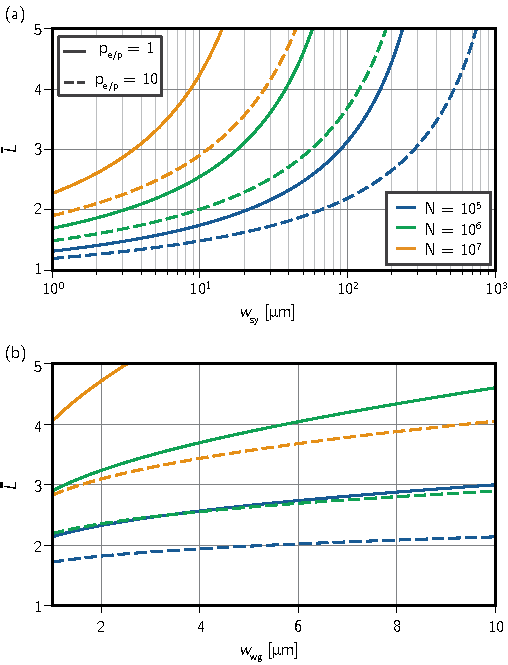
\includegraphics[width=8.6cm]{path_length__vs__width.pdf}
    \caption{Path length vs width.}
    \label{fig:path_length__vs__width}
\end{figure}
A key message of these plots is that it will be very difficult to integrate ten million neurons on a wafer while maintaining a short path length near 2.5. Even if only one million neurons per wafer are sought, multiple planes of active electronic circuits and passive photonic waveguides will make a significant difference in connectivity as quantified through network path length.

While Figs.\,\ref{fig:path_length__vs__width} only considers one or 10 planes, Fig.\,\ref{fig:num_planes} shows the number of planes required to achieve a path length of 2.5 as a function of the number of neurons on the wafer for several values of synapse and waveguide size. We will refer to Figs.\,\ref{fig:path_length__vs__width} and \ref{fig:num_planes} to guide the reasoning presented in the subsequent discussion of fabrication.
\begin{figure}
    \centering
    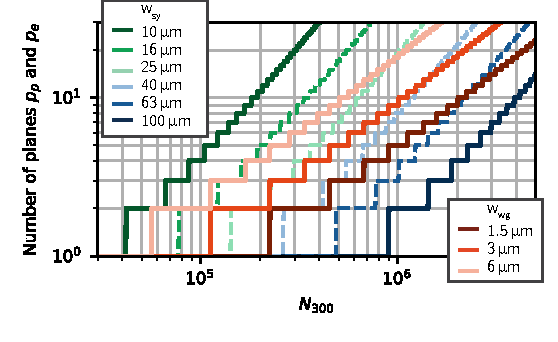
\includegraphics[width=8.6cm]{num_planes.pdf} 
    \caption{Num planes.}
    \label{fig:num_planes}
\end{figure}

\subsection{Fabrication Processes}
\label{sec:fabrication}
We assume 300\,mm silicon wafer processing. Wafer-scale integration has already been demonstrated for electronic neuromorphic systems \cite{schemmel2010wafer}. Still, even at this scale, reaching $10^6$ optoelectronic neurons per wafer is a tall order for either platform (figure \ref{fig:num_planes}). We choose this integration metric somewhat arbitrarily \textemdash it corresponds to $10^4$ wafers for a human cortex scale system. This is roughly the same order as the number of processing units in modern supercomputers. If this target is to be reached, 3D integration at some level will be necessary. From figure \ref{fig:num_planes}, it is clear that either platform will require a minimum of 4 photonic planes. Fortunately, photonic planes are quite amenable to 3D integration. Common waveguide materials include amorphous silicon (aSi), silicon nitride (SiN$_x$) and silicon oxynitride (SiO$_x$N$_y$). These dielectric materials can be deposited at low-temperature, enabling several multi-planar demonstrations \cite{shpa2015,sahu2015,chbu2017,zhli2018}. Additionally, low-temperature deposition makes such processes compatible with back-end CMOS fabrication. It should be noted that four photonic planes represents a best-case scenario, as wider waveguides have lower loss and only minimal reduction in average path length (fig \ref{fig:path_length__vs__width}). Six planes with 3\,\textmu m pitch \textcolor{blue}{(check)} were assumed in ref \cite{shainline2017superconducting}.

3D integration of active electronics is less straightforward, particularly for the semiconductor approach. 3D CMOS integration has been the subject of decades of research and is still plagued with uncertainty  \cite{lish2017}. The primary difficulty is that transistors made from amorphous or poly-crystalline materials are of inferior quality to their crystalline silicon counterparts \cite{}. Additionally, required high-temperature processing steps for dopant activation or contact anneals typically have a degrading effect on previous layers. For the semiconductor path, the best course of action may be to abandon 3D active electronics altogether in favor of simply reducing the footprint ($w_{sy}$) of synapses. We see again from figure \ref{fig:num_planes} that nearly $10^6$ neurons can be integrated on a single plane if each synapse is on the order of 10\,$\mu$m\,\times\,10\,$\mu$m. This may be a challenging benchmark to reach with high-functionality synapses implementing complex plasticity and dynamics. Subthreshold circuits that have embraced larger CMOS nodes for decreased variability, will likely need to adjust to more modern nodes, of which there is some precedent \cite{rupa2019}. Additionally, photodetectors will be on the micron scale and metal-insulator-metal (MIM) capacitors typically require about 1\,$\mu m^2$ per femtofarad, limiting the length of synaptic time constants on many chips \cite{indiveri2019importance}. Both of these elements would however be fabricated on separate planes from the MOSFETs.

Superconducting platforms would likely take the opposite approach, embracing 3D integration in the face of large device areas. Superconducting electronics, including the active element JJs, are routinely deposited at low temperatures ($<$\,180\,\textcelsius). Integrated circuits with two stacked planes of JJs have been demonstrated by two research laboratories \cite{tobo2019,anna2017}, along with multiple of planes of SNSPDs \cite{vema2012}. This is particularly important, as superconducting systems will not be able to reach $10^6$ neurons per wafer without 3D integration. A reasonable estimate for a superconducting synapse may be 30\,\textmu m on a side (Appendix \ref{apx:supporting_calculations}). Such a size would require 8 electronic planes. 

Lastly, we emphasize that even if $p_p = p_e = 1$, it is still possible to fabricate wafers with $10^6$ neurons, provided $\bar{k} = 100$, giving $\bar{L} = 3.5$. While this does not match the short path lengths of cognitive circuits in the brain, such a network is likely to have significant technological and scientific utility while offering an intermediate-term practical objective.

\subsection{Constructing Multi-Wafer Systems}
Given that neither system will scale to billions of neurons on a single wafer, many wafers ($\sim$10,000) will need to be connected together to support brain scale computing. A vision for a multi-wafer system is discussed in detail in reference \cite{shainline2020optoelectronic} for the SOENs platform. However, the basic geometry should be applicable to the semiconductor platform as well. Briefly, wafers are stacked to form highly inter-connected columns mimicking the modular structure of biological circuits. Columns are coupled to each other with inter-plane and free-space connections (both water and liquid helium are transparent at the wavelengths under consideration), but such connectivity is more sparse than that within a column. Finally, optical fibers can provide the most extreme long-distance connectivity. 

Achieving systems of this scale requires advances, particularly in wafer-scale circuit integration and system-level construction. A phenomenon akin to Moore's law, with ever-decreasing feature sizes enabling ever-higher integration density is unlikely to carry this concept forward, as many device sizes are limited by other physical considerations. Metrics related to number of synapses on a wafer, number of planes of integrated circuits, and number of wafers in a system may be more relevant to chart progress in neuromorphic supercomputing. Gradual progress may be possible by consistently scaling up, but it is difficult to envision this sustained trend without a powerful economic drive.  

\subsection{Power consumption and cooling}
\subsubsection{Cooling Systems}
Cooling systems will be a key component to either platform. The ability to remove heat is necessary to maintain normal circuit operation. This is particularly dramatic for superconducting electronics, in which the devices will lose superconductivity if the temperature rises above the critical temperature ($T_c$). Pending a revolutionary development in high-$T_c$ materials, superconducting neuromorphic systems will rely on niobium ($T_c = 9.3$K) or a material with a similarly low $T_c$. Liquid helium (4.2K) is the cryogen of choice for such temperatures. Cooling systems will add significantly to the power consumption of superconducting electronics. The power efficiency of a refrigeration system is measured by its specific power (the reciprocal of the coefficient of performance) \textcolor{red}{(sounds like a bit of jargon to the uninitiated)} \cite{}. The specific power gives the number of watts consumed by the refrigeration system for every watt of heat removed. The theoretical limit for specific power, given by the Carnot limit, is $\frac{T_H - T_C}{T_C}$. For liquid helium temperature (4.2\,K), the Carnot limit demands that at least $74$\,Watts of refrigeration power are required to remove every watt of heat produced on-chip if the system is operated in a 300\,K ambient. State-of-the-art systems have reached specific powers as low $250$\,W/W. Auspiciously, the most efficient refrigeration systems also tend to have the highest heat loads. Heat loads as high as 10\,kW at 4.4K have already been demonstrated by commercially available systems. Note that throughout this paper, we assume a more conservative specific power of $1000$\,W/W, representative of the smaller scale cryogenic systems used in most laboratories today. Overall, it does not appear that cryogenic capability will be an insurmountable obstacle towards large-scale superconducting neural systems.
\subsubsection{Power Limitations}
Modern supercomputers typically consume megawatts of power. Tianhe 2, for instance, requires 17.8\,MW for operation (and another 6.4\,MW for cooling) \cite{tolpygo2016superconductor}. If we thus assume a total power budget on the order of 10\,MW, we can analyze the trade-off between average firing rate and the number of neurons. We assume 1\,fJ of optical energy is required to initiate a firing event at each synapse and plot the maximum average frequency spiking frequency for several different optical link efficiencies in figure \ref{fig:freq_size}.

Power does not appear to be a limiting factor in achieving brain-scale and brain-speed optoelectronic networks. If the power resources of modern supercomputers were dedicated to a brain-scale optoelectronic neuromorphic system, average spiking rates on the order of 10\,kHz \textcolor{red}{(consider explaining how average of 10kHz comes from 1/f power spectral density up to 20\,MHz)} appear feasible even with relatively inefficient optical links. Such a system, if designed to cultivate similar activity as the human brain, would enable brain-scale simulation with time accelerated by four orders of magnitude.

\begin{figure}[h!]
    \centering
    \includegraphics[scale=1]{Pow.pdf}
    \caption{Tradeoff between size and average spiking frequency for a population of optoelectronic neurons with a power budget of 10 MW. Fan-out is $10^3$ and the optical energy needed at each synapse is assumed to be 1\,fJ (accounting for cooling in superconductor case). This likely would correspond to the limits of either superconductor or semiconductor neurons.}
    \label{fig:freq_size}
\end{figure}

Another factor to consider is power density. There is a maximum power density that can be handled by heat removal systems for both the semiconducting and superconducting case. In the semiconductor case, high-performance computing routinely generates power densities of hundreds of watts per square centimeter \cite{tolpygo2016superconductor}. A theoretical limit of around 1\,kW/cm$^2$ is postulated in ref \cite{zhirnov2003limits}. In contrast, superconducting systems will be required to operate at significantly lower power densities. Roughly 1 W/cm$^2$ is a conservative limit on the on-chip power density that can be cooled with liquid helium \cite{tolpygo2016superconductor}. Interestingly, superconducting optical links appear to be capable of dissipating about three orders of magnitude less energy per bit, approximately cancelling out the limited power density requirements of superconducting systems in comparison with semiconductors. In practice, it might well be the case that mature, sophisticated synapses and neurons will occupy so much area that these power density limitations will be of no consequence. For instance, even with link efficiencies of $1 \times 10^{-4}$, a synapse would require a lateral dimension of less than 30\,$\mu$m for power density considerations to limit spiking to less than 1\,GHz. Section \ref{sec:instantiation} argued that synapses are not likely to be smaller than this. However, it should also be noted that optoelectronic systems will have extremely nonuniform power dissipation across the chip/wafer, with most of the power being dissipated at the light sources. A more in-depth analysis is required to see if heat removal will be an issue near the light-sources in particular. Concerns about local heating may be assuaged with layouts that sufficiently shield and/or separate thermally sensitive devices from the light sources.

\section{\label{sec:conclusion}Conclusion}
The prospects of neuromorphic systems at the scale of the brain and beyond are tantalizing. The fan-out capability of optical communication, coupled with the computational power of electronic circuitry makes optoelectronic systems a promising framework for realizing these high ambitions. However, there is no technology platform that is ready to support optoelectronic spiking networks of the scale and sophistication of the human brain. Making this vision a reality will require breakthroughs at the device level, no matter which path is chosen. Beyond that, several different classes of devices must be integrated alongside each other, which further reduces the likelihood for success. Efficient, densely integrated light sources, waveguide-integrated detectors, local memory devices, and capable neuronal circuitry all must be consolidated onto a single platform. Candidates for all requisite devices can be proposed for either semiconducting or superconducting platforms, and the two systems may be capable of surprisingly similar performance. However, the technological paths toward achieving brain-scale systems with the two platforms diverge in important respects, and we have attempted to outline the main advantages and challenges for each.

Semiconductor platforms hold advantages in technological maturity, room-temperature operation, and perhaps speed. Spike rates in excess of 10 GHz may be feasible, but only for systems significantly smaller than the human brain. Semiconductor receivers can potentially operate with extremely low energies per spiking event (sub femto-joule), making them a worthy competitor of superconducting single photon detectors. However, these low energy receivers require significant optical power from integrated light sources. To achieve biological-scale fan-out, either very bright light sources, repeatering schemes (costing area and yield), or additional gain stages (costing power) will need to be included. In terms of neuronal computation, semiconductor neurons have already demonstrated impressive functionality and low-power operation that should be capable of integration with optical communication infrastructure, provided the long-standing challenges with CMOS-integrated III-V light sources can be overcome. Synaptic memory is a major open question, but a variety of non-volatile memory solutions have seen extensive investigation, and time will tell if one technology can meet the requirements we have laid out for brain-scale optoelectronic systems. Lastly, 3D integration of transistors, photodetectors, and memory may not be a feasible solution, meaning aggressive scaling of synaptic circuits while maintaining complex functionality is perhaps a better strategy. The fabrication processes for mature semiconductor neural systems may prove to be prohibitively complicated and heterogeneous, perhaps requiring different processing strategies for sources, detectors, and memories. If wafer-scale monolithic integration of these components cannot be achieved, and chip-scale die-stacking techniques are required, the outlook for achieving brain-scale systems becomes quite limited.

Superconducting optoelectronic neural systems suffer from a comparatively primitive fabrication ecosystem, but the incorporation of superconducting devices provides several intriguing attributes. Namely, SNSPD receivers place nearly the theoretical minimum burden on integrated light sources. This is coupled with the improvements in efficiency for light sources operating at cryogenic temperatures. These two factors make the large-scale integration of light sources appear far more achievable than in the semiconductor case\textemdash perhaps even opening the door to silicon as an active optical material. Driving these light sources with superconducting electronics, however, has yet to demonstrated with the performance required for this application. The implementation of such a circuit remains a major open challenge. For computation, superconducting neuronal circuits appear just as capable of implementing complex neuronal and synaptic behaviors as their CMOS counterparts, but will likely need to be designed with serial biasing in order to scale. Additionally, some speed advantages present in superconducting electronics will be negated by the response time of SNSPDs ($<$1\,GHz ). Of course, even if maximum spike rates are limited to 20 MHz, this would still represent a speed-up of about 4 orders of magnitude over biological systems. Memory seems to be a strength for the superconducting platform, as superconductivity provides new avenues of storing synaptic weights. Loop memory in particular may be capable of implementing plasticity mechanisms that operate with only the signals produced through normal network activity. Caution is in order here, however, as superconducting synaptic plasticity mechanisms have scarcely been explored. Additionally, 3D integration may yield more readily in the superconductor platform. Finally, the inconvenience of cryogenic cooling is a serious consideration, but power and heat removal estimations indicate this is unlikely to be a limiting factor for brain-scale systems. If all of these issues can be resolved, superconducting optoelectronic systems may actually require simpler manufacturing processes than the semiconductor approach, as the material ecosystem could potentially be relatively simple. Of course, superconducting foundries are far less developed than their semiconductor counterparts, which may negate these advantages in the near-term.

Finally, we would be remiss to paint the quest for neuromorphic supercomputing as only a question of hardware. The inner workings of the brain is the subject of intense investigation, and the emergent phenomena of cognition and consciousness remain taunting, increasingly lonely enigmas entrenched in the no-mans land between philosophy and science. Watershed breakthroughs in neuroscience and algorithmic development will be required for the discussed hardware platforms to ever have any practical applications, although they may be of use in helping to unravel some of these great mysterious. The question of whether it is imprudent to develop hardware before algorithms has pestered the field of neuromorphic computing since its inception. In this case, however, we believe that the length of development, rich opportunities for spin-off technologies, and inestimable potential make such hardware development well-worth pursuing even at this incipient state.  

\textbf{Targets and Necessary Developments}:
\newline
\newline
\textbf{Both}
\begin{itemize}
    \item Monolithic integration of light sources, detectors, memory devices, and active electronics
    \item At least 6 planes for photonic routing
    \item Wafer-scale processing
    \item Dense inter-wafer optical links

\end{itemize}

\textbf{Semi}
\begin{itemize}
    \item Demonstrate femto-joule optical receivers, ideally with low static power dissipation
    \item III/V integration with silicon electronics at the scale of 1 million light source/300 mm wafer
    \item Synapses and local plasticity mechanisms ideally reach 10 $\times$ 10 $\mu$m \textit{without sacrificing performance}
    \item Demonstrate a CMOS-integrated memory device capable of at least $10^{11}$ lifetime updates, picojoule update energy, update times of less than 100 ns and at least 4 bit precision - all with unobtrusive programming circuitry and tolerable variability
\end{itemize}

\textbf{Super}
\begin{itemize}
    \item \textbf{\textit{Either} }III/V integration with silicon \textbf{\textit{or}} cryogenic silicon light sources with at least $10^{-4}$ efficiency at the scale of 1 million light sources/300 mm wafer.
    \item Integrate an efficient driver that interfaces low-voltage superconducting electronics with semiconductor light sources
    \item Serial biasing or current-recycling schemes for current biasing of synapses and neurons
    \item Demonstration of local programming of loop memory
    \item Demonstrate 8 planes of Josephson junctions per wafer
    
\end{itemize}


\vspace{0.5em}
This is a contribution of NIST, an agency of the US government, not subject to copyright.
	
\newpage
\appendix

%\section{\label{apx:supporting_calculations}Supporting Calculations}
\section{Implementing Long Time Constants}

\section{Fan-In of Superconducting Neurons}
Fan-out and fan-in are primary considerations of neuronal circuits when assessing scaling potential. Consideration of fan-out has led to the proposal for photonic communication, which we have addressed in prior studies \cite{shbu2017,chbu2017,chbu2018,sh2018_ICRC,sh2019,sh2020}. The present study relates to models of dendrites and neurons, which perform fan-in through the synapto-dendritic tree. Analysis of the number of input connections to a dendrite or neuron cell body are therefore necessary to complete the study.

\begin{figure}[h!]
\includegraphics[width=8.6cm]{figures/_fig_apx__fan-in__circuits.pdf}
\captionof{figure}{\label{fig:fan-in__circuits}Caption of fig:fan-in circuits.}
\end{figure}
For synaptic or dendritic integration loops coupled directly to a dendritic or neuronal receiving loop, we would like to know how to choose the inductors shown in Fig.\,\ref{fig:fan-in__circuits}(a) so the applied flux stays in the appropriate operating range as the number of synaptic connections, $N$, is modified. This consideration will identify the limit of how many synapses can be coupled to a single dendrite or neuron\textemdash the fan-in limit. 

We have seen that the operation of a dendrite (or neuron cell body) is significantly shaped by the inductance of the DR loop. We would therefore like to be able to increase the number of synaptic connections without changing the total inductance of this loop. This total inductance is given by
\begin{equation}
\label{eq:fan-in__direct_input__si_inductance}
L^{\mathrm{nr1}}_{\mathrm{tot}} = \sum_i L^{\mathrm{nr1}}_i = N L^{\mathrm{nr1}}_0
\end{equation}
We would like $L^{\mathrm{nr1}}_{\mathrm{tot}}$ to be independent of $N$, which is possible with $L^{\mathrm{nr1}}_N = L^{\mathrm{nr1}}_0/N$. The total applied flux to the NR loop is given by
\begin{equation}
\label{eq:fan-in__direct_input__applied_flux}
\Phi_{\mathrm{a}}^{\mathrm{nr}} = \sum_i M_i^{\mathrm{si|nr}} \, I_i^{\mathrm{si}}.
\end{equation}
Suppose all SI loops contain a given current, $I_0^{\mathrm{si}}$. We would like the applied flux to the NR loop, $\Phi_{\mathrm{a}}^{\mathrm{nr}}$, to be independent of $N$:
\begin{equation}
\label{eq:fan-in__direct_input__flux_independent_of_N}
\frac{ \Phi_{\mathrm{a}}^{\mathrm{nr}} }{ I_0^{\mathrm{si}} } = \mathrm{cnst.} \neq f(N).
\end{equation}
In the case where all mutual inductors between synapses and the NR loop are equal,
\begin{equation}
\label{eq:fan-in__direct_input__flux_independent_of_N_2}
\frac{ \Phi_{\mathrm{a}}^{\mathrm{nr}}(N) }{ I_0^{\mathrm{si}} } = N\,k\,\sqrt{ L_N^{\mathrm{si2}} \, L_N^{\mathrm{nr1}}},
\end{equation}
where $L_N^{\mathrm{si2}}$ and $L_N^{\mathrm{nr1}}$ are the values of $L^{\mathrm{si2}}$ and $L^{\mathrm{nr1}}$ that we should choose for the SI loop output inductor when there are $N$ synapses coupled directly to the NR loop. We have seen above that we need $L_N^{\mathrm{nr1}} = L_0^{\mathrm{nr1}}/N$ to maintain the inductance of the NR loop. Therefore, in order for Eq.\,\ref{eq:fan-in__direct_input__flux_independent_of_N_2} to satisfy Eq.\,\ref{eq:fan-in__direct_input__flux_independent_of_N}, we must also have $L_N^{\mathrm{si2}} = L_0^{\mathrm{si2}}/N$.

This consideration does not explicitly identify a fan-in limit. This limit arises due to practical considerations related to making $L^{\mathrm{si2}}$ and $L^{\mathrm{nr1}}$ exceedingly small as $N$ grows large. Taking $L_0 \approx 1$\,pH as a rough lower limit on what we would like to fabricate, and $L_{\mathrm{tot}}^{\mathrm{nr}} \approx 20$\,pH, we see direct fan-in with this circuit design is limited to about 20. This limit can be straightforwardly overcome with an intermediate transformer collection coil, as shown in Fig.\,\ref{fig:fan-in__circuits}(b). In this configuration, the applied flux to the NR loop is
\begin{equation}
\label{eq:fan-in__transformer_collection__full}
\Phi_{\mathrm{a}}^{\mathrm{nr}} = \frac{ M^{\mathrm{nr|nt}} \, \sum_i M^{\mathrm{nt|si}}_i I_i^{\mathrm{si}} }{ \sum_i L^{\mathrm{nt1}}_i + L^{\mathrm{nt2}} + L^{\mathrm{nt3}} }.
\end{equation}
The mutual inductors are $M^{\mathrm{si|nt}} = k\sqrt{L^{\mathrm{si2}} \, L^{\mathrm{nt1}}}$ and $M^{\mathrm{nt|nr}} = k\sqrt{L^{\mathrm{nt3}} \, L^{\mathrm{nr1}}}$. We are interested in how this flux scales with the number $N$ of input synapses to the neuronal transformer (NT) loop. Consider the case where the mutual inductors between all synapses and the NT loop are identical: $M^{\mathrm{nt|si}}_i = M^{\mathrm{nt|si}} = k \sqrt{L^{\mathrm{si2}}L^{\mathrm{nt1}}}$, and $L^{\mathrm{nt1}}_i = L^{\mathrm{nt1}}$. Further assume all synaptic integration loops carry the same current $I^{\mathrm{si}}_i = I^{\mathrm{si}}_0$. Such a case is rare in operation but is sufficient for scaling analysis. Equation \ref{eq:fan-in__transformer_collection__full} becomes
\begin{equation}
\label{eq:fan-in__transformer_collection__identical_synapses}
\frac{ \Phi_{\mathrm{a}}^{\mathrm{nr}} }{ I^{\mathrm{si}}_0 } = \frac{ M^{\mathrm{nr|nt}} \, M^{\mathrm{nt|si}} }{ L^{\mathrm{nt1}} } \left( 1 + \frac{ L^{\mathrm{nt2}} + L^{\mathrm{nt3}} } { N L^{\mathrm{nt1}} } \right)^{-1}.
\end{equation}
From Eq.\,\ref{eq:fan-in__transformer_collection__identical_synapses} one can see the ratio of flux in the NR loop to current in each of the SI loop becomes nearly independent of $N$ for large $N$. 

We can further elucidate the scaling by noting that the circuit of Fig.\,\ref{fig:fan-in__circuits}(b) has three types of inductors. Transformers are likely to be asymmetrical, with a larger inductor coupling flux into a smaller inductor to achieve a reasonable mutual inductance with a modest receiving loop inductance. We can therefore specify $M^{\mathrm{nr|nt}} = M^{\mathrm{nt|si}} = k \sqrt{ L_{\mathrm{m}} \, L_{\mathrm{s}}}$, where $L_{\mathrm{m}}$ refers to a medium-sized inductor, on the order of 100\,pH, and $L_{\mathrm{s}}$ is a small inductor, on the order of 10\,pH. Thus, $L^{\mathrm{si2}} = L^{\mathrm{nt3}} = L_{\mathrm{m}}$, and $L^{\mathrm{nt1}} = L^{\mathrm{nr1}} = L_{\mathrm{s}}$. The inductor $L^{\mathrm{nt2}}$ is a parasitic inductance that we anticipate being unavoidable in the fabrication of a large NT loop. We assume $L^{\mathrm{nt2}} = L_{\mathrm{m}}$. The third inductance in the circuit is $L^{\mathrm{si1}}$, a large self-inductance unassociated with a transformer, which we label as a big inductor, $L_{\mathrm{b}}$. This inductance will likely be in the range of 10\,nH - 10\,\textmu H, and for the sake of this analysis consideration of the value of 10\,nH is sufficient. The large value of this inductance gives the synapse (or dendrite in the case of a DI loop) an analog response. In hardware, such large values are made possible by high-kinetic-inductance materials \cite{}, wherein the inductance is a result of the motion of the current-carrying cooper pairs rather than the coupling between a current and the magnetic field it produces. With these simplifications, Eq.\,\ref{eq:fan-in__transformer_collection__identical_synapses} becomes
\begin{equation}
\label{eq:fan-in__transformer_collection__three_inductances}
\frac{ \Phi_{\mathrm{a}}^{\mathrm{nr}} }{ I^{\mathrm{si}}_0 } = k^2 L_{\mathrm{m}} \left( 1 + \frac{2L_{\mathrm{m}}}{NL_{\mathrm{s}}} \right)^{-1}.
\end{equation}
The term $2L_{\mathrm{m}}/NL_{\mathrm{s}}$ is of order unity when $N\approx 10$ and becomes small when $N \approx 100$. In the large-$N$ limit we can make the approximation
\begin{equation}
\label{eq:fan-in__transformer_collection__large_N}
\frac{ \Phi_{\mathrm{a}}^{\mathrm{nr}} }{ I^{\mathrm{si}}_0 } \approx k^2 L_{\mathrm{m}} \left( 1 - \epsilon \right) + \mathcal{O}(\epsilon^2),
\end{equation}
where
\begin{equation}
\label{eq:fan-in__transformer_collection__epsilon}
\epsilon \equiv \frac{ 2L_{\mathrm{m}} }{ N L_{\mathrm{s}} }.
\end{equation}
Thus, a dendrite or neuron receiving input from $N$ synapses or dendrites, each containing current $I^{\mathrm{si}}_0$ in their integration loop, receives flux that is independent of $N$ to leading order. This appears to be an advantageous fan-in scenario, made possible by the shared transformer collection coil. We have seen above that roughly 20 synapses or dendrites can be directly coupled to a receiving loop. When 20 synapses or dendrites are coupled to a transformer collection coil, $\epsilon$ is on the order of unity, and therefore not sufficiently small as to be neglected for design purposes. Yet in this case the total applied flux to the receiving loop will be within a factor of two of the directly coupled case. Above 20 inputs, the situation only improves with $N$. Therefore, it appears fan-in is achievable for any number of inputs. 

To gain further confidence in this conclusion, we must consider the ability of a collection of $N$ inputs to drive a dendrite or neuron to threshold as well as the cross talk between the inputs. Let us refer to the value of flux that will drive the neuron above threshold as $\Phi^{\mathrm{nr}}_{\mathrm{th}}$. As discussed in Sec.\,\ref{sec:dendrites}, this value is determined by circuit parameters and current biases, which are independent of the number of inputs. As a model of scaling potential, we would like to know what value of $I^{\mathrm{si}}_{\mathrm{th}}$ is required in each synapse of a homogeneous point neuron to achieve $\Phi^{\mathrm{nr}}_{\mathrm{th}}$. In the large-$N$ limit, we can straightforwardly rearrange Eq.\,\ref{eq:fan-in__transformer_collection__large_N} and apply the binomial approximation to arrive at
\begin{equation}
\label{eq:fan-in__transformer_collection__threshold_current}
I^{\mathrm{nr}}_{\mathrm{th}} = \frac{1+\epsilon}{k^2 L_{\mathrm{m}}} \Phi^{\mathrm{nr}}_{\mathrm{th}}.
\end{equation}
Again we find the quantity of interest is independent of $N$ to leading order. The factor proportional to $\epsilon$ must be accounted for in design, but the scaling with large $N$ is favorable. 

Consider the smallest number of synapses capable of achieving the threshold flux. There are $N$ synapses on the transformer collection coil, and we seek the number $P$ of them such that when those synapses reach saturation ($I^{\mathrm{si}} = I^{\mathrm{si}}_{\mathrm{sat}}$) the total applied flux reaches threshold ($\Phi^{\mathrm{nr}}_{\mathrm{a}} = \Phi^{\mathrm{nr}}_{\mathrm{th}}$). Here we begin with the exact expression of Eq.\,\ref{eq:fan-in__transformer_collection__full} rather than making a large-$N$ approximation. Assuming again identical synapses, and taking inductors to be small ($L_{\mathrm{s}}$), medium ($L_{\mathrm{m}}$), or big ($L_{\mathrm{b}}$), we can calculate the fraction of saturated synapses required to reach threshold, assuming all other synapses have zero integrated current.
\begin{equation}
\label{eq:fan-in__transformer_collection__fraction_for_threshold}
\frac{P}{N} = \frac{ \Phi^{\mathrm{nr}}_{\mathrm{th}} }{ k^2  I^{\mathrm{si}}_{\mathrm{sat}} } \left( \frac{1}{ L_{\mathrm{m}} } + \frac{2}{ N L_{\mathrm{s}} }  \right).
\end{equation}
The leading term is again independent of $N$, and the correction term recedes as $1/N$. The fraction of synapses that must be active to drive a dendrite or neuron above threshold converges to a fixed value at large $N$. Using realistic numbers, in the small-$N$ limit, $P/N \approx 0.1$, and in the large-$N$ limit, $P/N \approx 0.03$.

Finally, we consider cross talk between synapses or dendrites coupled to a common transformer receiving loop. Consider an NT loop with $N$ synaptic connections, $n$ of which contain current $I^{\mathrm{si}}_0$ in their SI loop. A net current will be induced in the NT loop due to the flux from the synapses,
\begin{equation}
\label{eq:fan-in__transformer_collection__I_nt}
I^{\mathrm{nt}} = \frac{\Phi^{\mathrm{nt}}}{L^{\mathrm{nt}}}\rightarrow \frac{ n k \sqrt{L_{\mathrm{m}}\,L_{\mathrm{s}}}}{NL_{\mathrm{s}}+2L_{\mathrm{m}}},
\end{equation}
and this current will induce a current in each SI loop, $I^{\mathrm{si}}_{\mathrm{ind}} = \Phi^{\mathrm{si}}_{\mathrm{ind}}/L^{\mathrm{si}} = M^{\mathrm{si|nt}}I^{\mathrm{nt}}/(L^{\mathrm{si1}}+L^{\mathrm{si2}})$. Making the association $L^{\mathrm{si1}} = L_{\mathrm{b}}$, and approximating $L_{\mathrm{b}} + L_{\mathrm{m}} \approx L_{\mathrm{b}}$, we find the ratio of the induced current in each SI loop to the integrated current in one of the $n$ active synapses is
\begin{equation}
\label{eq:fan-in__transformer_collection__cross_talk}
\frac{I^{\mathrm{si}}_{\mathrm{ind}}}{I^{\mathrm{si}}_0} = \frac{n}{N}\frac{k^2L_{\mathrm{m}}}{L_{\mathrm{b}}}\left( 1+\epsilon \right)^{-1}.
\end{equation}
As stated above, $L_{\mathrm{b}}$ is likely to be in the range of 10\,nH - 10\,\textmu H, while $L_{\mathrm{m}}$ is on the order of 100\,pH. The term $L_{\mathrm{m}}/L_{\mathrm{b}}$ will be less than 0.01, and typically much less than this value. The worst case for cross talk occurs when all synapses contain integrated current $I^{\mathrm{si}}_0$ so $n = N$. For rough estimate of scaling, we can ignore the $k^2$ term and the $\epsilon$ term, both of which act to reduce the cross talk. In the extreme limit where all $N$ SI loops contain the saturated current $I^{\mathrm{si}}_{\mathrm{sat}}$, the fraction of current induced in each loop scales as
\begin{equation}
\label{eq:fan-in__transformer_collection__cross_talk__worst_case}
\frac{I^{\mathrm{si}}_{\mathrm{ind}}}{I^{\mathrm{si}}_{\mathrm{sat}}} \approx \frac{L_{\mathrm{m}}}{L_{\mathrm{b}}} < 10^{-3}.
\end{equation}
The key feature of loop neurons regarding cross talk is that the SI loop inductance is large, yet a small fraction of this inductance feeds into the mutual inductor. The asymmetry of the inductances between $L^{\mathrm{dr}}$ and $L^{\mathrm{di}}$ is necessary to reduce cross talk. This inductance imbalance is also precisely what enables the dendrite to produce an analog output. If one uses a dendrite or neuron to produce a binary, single-flux-quantum output, the inductance of the DI loop will be on the same order as the inductance of the inductors in the transformers, and cross talk will cause a problem for fan-in. However, leveraging high-kinetic-inductance materials and analog synapses and dendrites, cross talk is not a problem, and fan-in behaves favorably from a small number of inputs up to large $N$.

\section{Area Estimate of Superconducting Neurons}
Based on the typical SQUID design criterion we expect $\beta_{\mathrm{L}} = 2LI_c/\Phi_0 = 1$ \cite{clbr2006}. The scaling of a washer-type inductor informs us that $L \approx \mu_0 r$, where $r$ is the inner diameter. The energy for a SQUID to produce a pair of fluxons is given by $E_{\mathrm{sq}} = 2E_{\mathrm{j}} = 2 \langle I_b \rangle \Phi_0 \approx 2 I_c \Phi_0$. We can combine these expression to arrive at $w_{\mathrm{sq}} = 2\Phi_0^2/\mu_0 E_{\mathrm{sq}}$.

\begin{figure}[!h]
    \centering
    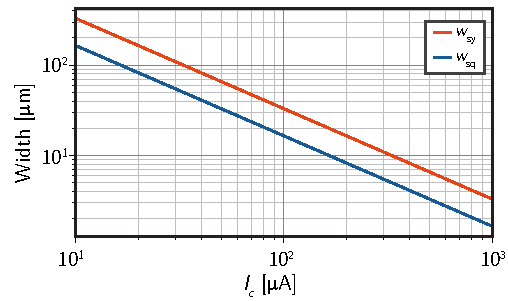
\includegraphics[width=8.6cm]{squid_size.pdf}
    \caption{Squid size.}
    \label{fig:squid_size}
\end{figure}






\bibliographystyle{unsrt}
\bibliography{bib}
\end{document}
